\documentclass[aspectratio=169]{beamer}
\usetheme{Madrid}
\usecolortheme{beaver}

%draw graphics
\usepackage{tikz, pgfplots}
\usetikzlibrary{positioning}

\usepackage[english]{babel}
%show outline before start a section
\newif\ifshowtoc
\showtoctrue% toggles to show the toc
\AtBeginSection{%
\ifshowtoc
\begin{frame}{Outline}
    \tableofcontents[currentsection, subsectionstyle=show/show/hide]
\end{frame}
\fi
}


\title{Computer Vision: Face Detection \& Recognition}
\author{Moatasem Gamal}

\institute{FCAI BSU}

\begin{document}
\maketitle
\part{Face Detection}
\begin{frame}{Part I: Face Detection}
    \tableofcontents
\end{frame}

\section{What is Face Detection}
\begin{frame}{What is Face Detection}
    \begin{itemize}
        \item     \textbf{Object detection} is one of the computer technologies that is connected to image processing and computer vision. It is concerned with detecting instances of an object such as human faces, buildings, trees, cars, etc. \cite{FaceDetectionGreatLearning:2023}
        \item The primary aim of face detection algorithms is to determine whether there is any face in an image or not.
    \end{itemize}
\end{frame}
\section{Face Detection Applications}
\begin{frame}{Face Detection Applications}
    \begin{itemize}
        \item Auto focus using face detection in Smart Phones
        \item People Search in Search Engines like MS Bing
    \end{itemize}
\end{frame}
\subsection{Auto focus using face detection in Smart Phones}

\subsection{People Search in Search Engines like MS Bing}
\begin{frame}{People Search in Search Engines like MS Bing}
    \includegraphics<1>[width=0.99\linewidth]{assets/figures/gates-bing-search01.png}
    \includegraphics<2>[width=0.99\linewidth]{assets/figures/gates-bing-search02.png}
    \includegraphics<3>[width=0.99\linewidth]{assets/figures/gates-bing-search03.png}
    \includegraphics<4>[width=0.99\linewidth]{assets/figures/gates-bing-search04.png}
\end{frame}
\section{Viola-Jones Algorithm}
\begin{frame}{Viola-Jones Algorithm}
    \begin{itemize}
        \item Viola Jones algorithm is named after two computer vision researchers who proposed the method in 2001, Paul Viola and Michael Jones in their paper, “Rapid Object Detection using a Boosted Cascade of Simple Features”\cite{990517}.
        \item The Viola Jones algorithm has four main steps, which we shall discuss in the sections to follow:
              \begin{itemize}
                  \item Creating an integral image
                  \item Selecting Haar-like features
                  \item Running AdaBoost training
                  \item Creating classifier cascades
              \end{itemize}
              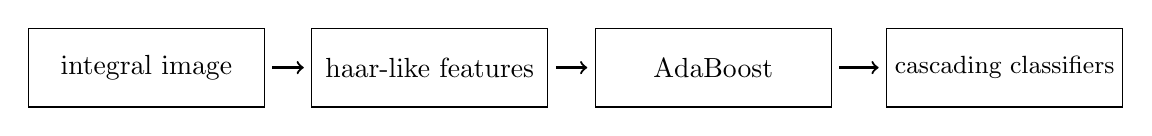
\begin{tikzpicture}
                  \draw (0,0) rectangle (3, 1);
                  \draw[->, thick] (3.1, .5) -- (3.5,0.5);
                  \draw node at (1.5, 0.5) {integral image};

                  \draw (3.6, 0) rectangle (6.6, 1);
                  \draw[->, thick] (6.7, 0.5) -- (7.1, 0.5);
                  \draw node at (5.1, 0.5) {haar-like features};

                  \draw (7.2, 0) rectangle (10.2, 1);
                  \draw[->, thick] (10.3, 0.5) -- (10.8, 0.5);
                  \draw node at (8.7, 0.5) {AdaBoost};

                  \draw (10.9, 0) rectangle (13.9, 1);
                  \draw node at (12.4, 0.5) {\small{cascading classifiers}};
              \end{tikzpicture}
        \item this algorithm works on grayscale image
    \end{itemize}
\end{frame}
\section{Haar-like features}
\begin{frame}{Haar-like features}
    \begin{itemize}
        \item Haar-like features are digital image features used in object recognition.
        \item There are 3 types of Haar-like features that Viola and Jones identified in their research:
              \begin{figure}[h]
                  \centering
                  \includegraphics[width=0.3\linewidth]{assets/figures/haar-like-features.png}
              \end{figure}
        \item we can divide a group of pixels into two categories, white (1) and black (-1)
        \item different sizes for the same feature
    \end{itemize}
\end{frame}
\subsection{Calculate haar-like features}
\begin{frame}{Calculate haar-like features}
    for every image apply sub-windows of 24$\times$24:
    \begin{equation}
        \delta = white_{region} - black_{region}
    \end{equation}
    Example: \\
    \begin{minipage}{0.3\linewidth}
        \centering
        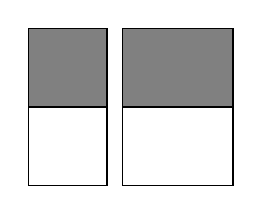
\begin{tikzpicture}
            \draw[fill=gray] (0,0) rectangle (1,1);
            \draw[fill=white] (0,0) rectangle (1,-1);

            \draw[fill=gray] (1.2,0) rectangle (2.6,1);
            \draw[fill=white] (1.2,0) rectangle (2.6,-1);
        \end{tikzpicture}
    \end{minipage}
    \begin{minipage}{0.6\linewidth}
        \centering
        \begin{figure}
            \includegraphics[width=.65\linewidth]{assets/figures/img-pixels.png}
            \caption{src: Haar Feature In Detail (youtube) \cite{HaarFeaturesIndetail}}
        \end{figure}
    \end{minipage}
\end{frame}
\subsection{Example on haar-like features}
\begin{frame}{Example on haar-like features}
    \centering
    \includegraphics<1>[width=0.85\linewidth]{assets/figures/haar-appleid01.png}
    \includegraphics<2>[width=0.85\linewidth]{assets/figures/haar-appleid02.png}
    \onslide<3->{
        Extracting a 180,000+ features \\
        \includegraphics<3>[width=0.7\linewidth]{assets/figures/haar-applied03.png}
    }
\end{frame}
\section{Integral Image}
\begin{frame}{Integral Image}
    We Use Integral Image approach to Running time \\ \vspace{0.5cm}
    \begin{figure}
        \centering
        \includegraphics<1>[width=0.8\linewidth]{assets/figures/integral-image01.png}
        \includegraphics<2>[width=0.8\linewidth]{assets/figures/integral-image02.png}
        \caption{src: CVision Viola Jones (youtube) \cite{CVisionViolaJones}}
    \end{figure}
\end{frame}
\section{AdaBoost}
\begin{frame}{AdaBoost}
    \begin{itemize}
        \item Eliminate the irrelevant Features
        \item with this technique, their final set of useful features got reduced to approx 6000
    \end{itemize}
\end{frame}
\section{Cascade Classifier}
\begin{frame}{Cascade Classifier}
    \begin{itemize}
        \item A set of week classifiers are combined to form a strong classifier.
        \item The more week classifier combined, the stronger the cascade classifier will be.
    \end{itemize}
    \begin{figure}
        \includegraphics[width=0.7\linewidth]{assets/figures/cascade-classifier.png}
    \end{figure}
\end{frame}

\begin{frame}{References}
    \bibliography{references}
    \bibliographystyle{plain}
\end{frame}
\end{document}

